%%%%%%%%%%%%%%%%%%%%%%%%%%%%%%%%%%%%%%%%%%%%%%%%%%%%%%%%%%%%%%%%%%%%%%%%%%%%%
% BENCHMARKING AI FACTORIES ON MELUXINA
% Technical Report - EUMaster4HPC Student Challenge 2025-2026
%%%%%%%%%%%%%%%%%%%%%%%%%%%%%%%%%%%%%%%%%%%%%%%%%%%%%%%%%%%%%%%%%%%%%%%%%%%%%

\documentclass[11pt,a4paper]{article}

% --- Packages ---
\usepackage[utf8]{inputenc}
\usepackage[T1]{fontenc}
\usepackage[english]{babel}
\usepackage{geometry}
\geometry{left=2.5cm, right=2.5cm, top=2.5cm, bottom=2.5cm}

\usepackage{graphicx}
\usepackage{booktabs}
\usepackage{tabularx}
\usepackage{longtable}
\usepackage{xcolor}
\usepackage{hyperref}
\usepackage{amsmath}
\usepackage{fancyhdr}
\usepackage{float}
\usepackage{caption}
\usepackage{enumitem}
\usepackage{tikz}
\usetikzlibrary{shapes.geometric, arrows.meta, positioning, fit}

% --- Hyperref Configuration ---
\hypersetup{
    colorlinks=true,
    linkcolor=blue!70!black,
    urlcolor=blue!70!black,
    citecolor=blue!70!black,
    pdftitle={Benchmarking AI Factories on MeluXina}
}

% --- Header/Footer ---
\pagestyle{fancy}
\fancyhf{}
\fancyhead[L]{\textit{Benchmarking AI Factories on MeluXina}}
\fancyhead[R]{\textit{EUMaster4HPC 2025-2026}}
\fancyfoot[C]{\thepage}
\renewcommand{\headrulewidth}{0.4pt}
\renewcommand{\footrulewidth}{0.4pt}

% --- Title ---
\title{%
    \vspace{-1cm}
    \textbf{Benchmarking AI Factories on MeluXina}\\[0.5cm]
    \large A Modular Framework for Reproducible AI Workload Evaluation on EuroHPC Systems\\[0.3cm]
    \normalsize EUMaster4HPC Student Challenge 2025-2026
}
\author{%
    Team 11
}
\date{January 2026}

\begin{document}

\maketitle

\begin{abstract}
This technical report presents a Python-based benchmarking framework designed for evaluating AI Factory components on the MeluXina supercomputer. The framework addresses the need for reproducible, modular, and scalable benchmarking of AI workloads---including LLM inference servers and object storage systems---in HPC environments. The system leverages SLURM for job orchestration, Apptainer for containerization, and Prometheus for metrics collection. This document details the system architecture, core components, execution flow, and performance analysis.
\end{abstract}

\tableofcontents
\newpage

%%%%%%%%%%%%%%%%%%%%%%%%%%%%%%%%%%%%%%%%%%%%%%%%%%%%%%%%%%%%%%%%%%%%%%%%%%%%%
% SECTION 1: INTRODUCTION
%%%%%%%%%%%%%%%%%%%%%%%%%%%%%%%%%%%%%%%%%%%%%%%%%%%%%%%%%%%%%%%%%%%%%%%%%%%%%
\section{Executive Summary and Introduction}
\label{sec:introduction}

\subsection{Context: AI Factories in Europe}

The European High-Performance Computing Joint Undertaking (EuroHPC JU) has established a network of petascale and pre-exascale supercomputers across Europe. Among these systems, MeluXina---hosted at LuxProvide in Luxembourg---represents critical infrastructure for AI, machine learning, and deep learning applications.

The concept of ``AI Factories'' has emerged as a paradigm for organizing computational resources dedicated to AI training, inference, and data processing at scale. These factories integrate:

\begin{itemize}[noitemsep]
    \item \textbf{Inference Servers:} High-throughput model serving (vLLM, TensorRT-LLM, Triton)
    \item \textbf{Object Storage:} Scalable data lakes for artifacts (MinIO, Ceph)
    \item \textbf{Vector Databases:} Semantic search support (ChromaDB, Milvus)
    \item \textbf{Orchestration:} Workflow management and scheduling
\end{itemize}

However, the lack of standardized benchmarking methodologies for these components on HPC systems presents a significant challenge.

\subsection{Project Objective}

This project delivers a \textbf{modular, reproducible, and scalable} benchmarking framework:

\begin{description}[style=nextline]
    \item[Modular Architecture] Four-module design (Servers, Clients, Monitors, Loggers) with abstract base classes enabling extension to new services.
    
    \item[Reproducible Execution] YAML-based ``Recipe'' configuration files capture complete experiment specifications.
    
    \item[Scalable Deployment] Native SLURM integration supports multi-node deployments with configurable parallelism.
    
    \item[HPC-Native Design] First-class Apptainer container support and module-based environment management.
\end{description}

%%%%%%%%%%%%%%%%%%%%%%%%%%%%%%%%%%%%%%%%%%%%%%%%%%%%%%%%%%%%%%%%%%%%%%%%%%%%%
% SECTION 2: SYSTEM ARCHITECTURE
%%%%%%%%%%%%%%%%%%%%%%%%%%%%%%%%%%%%%%%%%%%%%%%%%%%%%%%%%%%%%%%%%%%%%%%%%%%%%
\section{System Architecture}
\label{sec:architecture}

\subsection{High-Level Overview}

The benchmarking framework implements a layered architecture comprising four principal modules orchestrated by a central \texttt{BenchmarkManager} component. Figure~\ref{fig:architecture} illustrates the system design.

\begin{figure}[H]
\centering
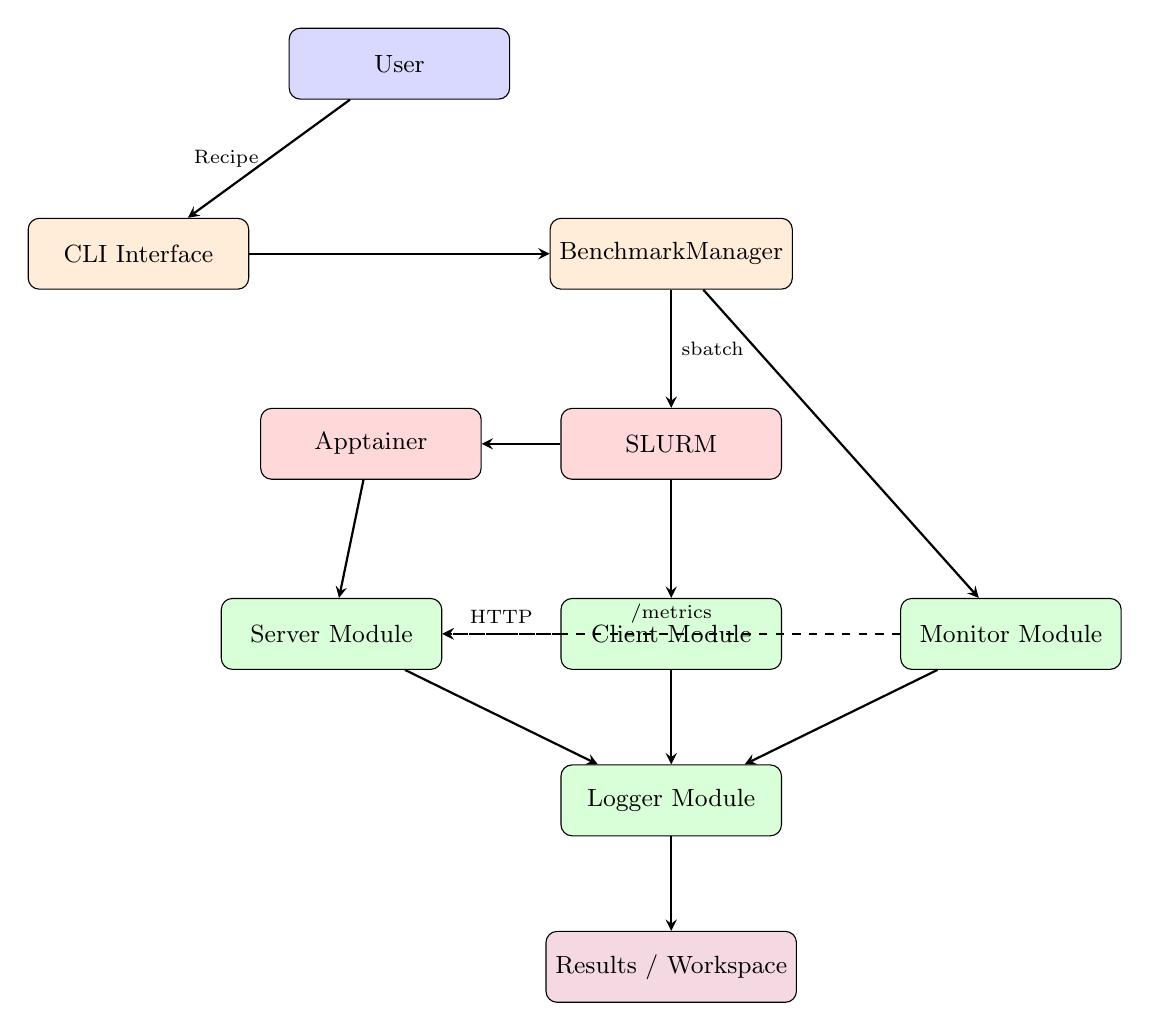
\begin{tikzpicture}[
    node distance=1.2cm and 2cm,
    box/.style={rectangle, draw, rounded corners, minimum width=2.8cm, minimum height=0.9cm, text centered, font=\small},
    userbox/.style={box, fill=blue!15},
    intbox/.style={box, fill=orange!15},
    hpcbox/.style={box, fill=red!15},
    compbox/.style={box, fill=green!15},
    storbox/.style={box, fill=purple!15},
    arrow/.style={->, >=stealth, thick},
    dashedarrow/.style={->, >=stealth, thick, dashed}
]

% Row 1: User
\node[userbox] (user) {User};

% Row 2: Interface
\node[intbox, below left=1.5cm and 0.5cm of user] (cli) {CLI Interface};
\node[intbox, below right=1.5cm and 0.5cm of user] (bm) {BenchmarkManager};

% Row 3: HPC
\node[hpcbox, below=1.5cm of bm] (slurm) {SLURM};
\node[hpcbox, left=1cm of slurm] (apptainer) {Apptainer};

% Row 4: Compute modules
\node[compbox, below left=1.5cm and 1.5cm of slurm] (server) {Server Module};
\node[compbox, below=1.5cm of slurm] (client) {Client Module};
\node[compbox, below right=1.5cm and 1.5cm of slurm] (monitor) {Monitor Module};

% Row 5: Logger + Storage
\node[compbox, below=1.2cm of client] (logger) {Logger Module};
\node[storbox, below=1.2cm of logger] (results) {Results / Workspace};

% Arrows
\draw[arrow] (user) -- node[left, font=\scriptsize] {Recipe} (cli);
\draw[arrow] (cli) -- (bm);
\draw[arrow] (bm) -- node[right, font=\scriptsize] {sbatch} (slurm);
\draw[arrow] (slurm) -- (apptainer);
\draw[arrow] (apptainer) -- (server);
\draw[arrow] (slurm) -- (client);
\draw[arrow] (bm) -- (monitor);

\draw[dashedarrow] (client) -- node[above, font=\scriptsize] {HTTP} (server);
\draw[dashedarrow] (monitor) -- node[above, font=\scriptsize] {/metrics} (server);

\draw[arrow] (server) -- (logger);
\draw[arrow] (client) -- (logger);
\draw[arrow] (monitor) -- (logger);
\draw[arrow] (logger) -- (results);

\end{tikzpicture}
\caption{High-level system architecture showing User, Interface, HPC, Compute, and Storage layers.}
\label{fig:architecture}
\end{figure}

\subsubsection{Module Responsibilities}

\begin{itemize}{
    \item \textbf{Server Module:} Encapsulates long-running services such as vLLM inference servers or MinIO object storage. Servers are launched via executors, monitored for health via HTTP healthchecks, and expose Prometheus-compatible metrics endpoints.

    \item \textbf{Client Module:} Implements load generation workloads that stress-test servers. Clients execute configurable request patterns with concurrent workers, collecting latency distributions and throughput metrics.
    
    \item \textbf{Monitor Module:} Performs pull-based metrics scraping from server endpoints at configurable intervals. The \texttt{PrometheusMonitor} parses Prometheus exposition format and persists time-series data to JSON files.
    
    \item \textbf{Logger Module:} Provides thread-safe, centralized logging for distributed components. Supports JSON and plaintext formats.
}
\end{itemize}

\subsection{HPC Integration}

The framework integrates with MeluXina through multiple touchpoints:

\begin{enumerate}[noitemsep]
    \item \textbf{Environment Modules:} The \texttt{run\_benchmark.sh} script initializes Lmod, loading Python and Apptainer modules.
    
    \item \textbf{Scratch Filesystem:} All workspace directories use scratch storage for high-performance I/O.
    
    \item \textbf{GPU Partition:} SLURM job scripts target the GPU partition with A100 allocation.
\end{enumerate}

\subsubsection{SLURM Workload Manager Interaction}

The \texttt{SlurmExecutor} class provides programmatic SLURM job management. Upon receiving a command string, the executor first checks whether an Apptainer container image is configured; if so, it wraps the command inside an \texttt{apptainer exec} invocation. The executor then writes the command to a temporary shell script, constructs a complete \texttt{sbatch} command line with configured resource parameters (nodes, GPUs, time limit, account), and submits the job via subprocess. The returned job ID is stored for subsequent status queries or cancellation.

The executor maintains internal state tracking the current job ID, enabling the \texttt{status()} method to query SLURM via \texttt{squeue} and return the job state. The \texttt{stop()} method issues \texttt{scancel} to terminate jobs gracefully.

%%%%%%%%%%%%%%%%%%%%%%%%%%%%%%%%%%%%%%%%%%%%%%%%%%%%%%%%%%%%%%%%%%%%%%%%%%%%%
% SECTION 3: CORE COMPONENTS
%%%%%%%%%%%%%%%%%%%%%%%%%%%%%%%%%%%%%%%%%%%%%%%%%%%%%%%%%%%%%%%%%%%%%%%%%%%%%
\section{Core Components and Design}
\label{sec:components}

This section analyzes the framework's core components, examining object-oriented design patterns and implementation strategies.

\subsection{Abstract Base Classes and Contracts}

The framework establishes a contract-based architecture through three abstract base classes in \texttt{src/Core/abstracts.py}.

\subsubsection{The Executor Contract}

The \texttt{Executor} abstract class defines the universal interface for all execution backends. It mandates three methods: \texttt{run()} accepts a command payload and returns an identifier, \texttt{stop()} terminates execution, and \texttt{status()} returns current state. This abstraction decouples orchestration logic from specific execution mechanisms.

Four concrete executors implement this contract:

\begin{table}[H]
\centering
\caption{Executor implementations and their behaviors}
\label{tab:executors}
\begin{tabularx}{\textwidth}{@{}l X@{}}
\toprule
\textbf{Executor} & \textbf{Behavior} \\
\midrule
\texttt{SlurmExecutor} & Submits jobs to SLURM via \texttt{sbatch}, tracks job IDs, queries status via \texttt{squeue}, cancels via \texttt{scancel}. Supports GPU allocation and Apptainer wrapping. \\
\texttt{ApptainerExecutor} & Launches commands inside Apptainer containers. \\
\texttt{ProcessExecutor} & Executes shell commands as subprocesses with process group isolation. Spawns daemon threads to stream output to the logger. \\
\texttt{WorkloadExecutor} & Runs in-process Python workloads on background threads. Retrieves runner functions from the workload registry. \\
\bottomrule
\end{tabularx}
\end{table}

\subsubsection{Monitor and Logger Contracts}

The \texttt{Monitor} abstract class requires \texttt{start()}, \texttt{collect()}, and \texttt{stop()} methods, establishing a lifecycle protocol for metrics collection. The \texttt{Logger} abstract class mandates \texttt{log()} for message recording and \texttt{export()} for persistence.

\subsection{The Service Composition Layer}

The \texttt{Service} class implements the \textbf{Composition Pattern}, assembling an executor, optional monitor, and optional logger into a cohesive unit. When \texttt{start()} is invoked, the service first logs the startup event, activates the monitor's background scraping, and delegates command execution to the executor. The \texttt{stop()} method reverses this sequence with exception handling to prevent cascading failures.

\subsection{Server and Client Modules}

\begin{itemize}{
    \item The \texttt{Server} class extends \texttt{Service} with server-specific behavior, storing command configuration and implementing \texttt{\_resolve\_command()} to normalize input (string or dictionary). The \texttt{start\_service()} method resolves the command and delegates to the parent.
    
    \item The \texttt{Client} class extends \texttt{Service} for workload generation, storing workload specifications and using \texttt{\_resolve\_payload()} to determine executor input. When executor type is ``workload'', the entire configuration dictionary passes to the \texttt{WorkloadExecutor}.
    
    \item The \texttt{BenchmarkManager} supports client scaling through the \texttt{instances} field. 
    
    The \texttt{\_expand\_client\_specs()} method creates deep copies for each instance, appending indices to IDs (e.g., ``vllm-loadgen-1'', ``vllm-loadgen-2'').
}
\end{itemize}

\subsection{Monitor Module: Prometheus Metrics Collection}

The \texttt{PrometheusMonitor} implements a pull-based scraping model. Upon initialization, it receives scrape targets, intervals, and output paths.

When \texttt{start()} is called, the monitor spawns a daemon thread running a scrape loop. This loop invokes \texttt{collect()}, then waits on a threading Event with the scrape interval as timeout. The Event-based wait allows immediate termination when \texttt{stop()} signals.

The \texttt{collect()} method iterates over targets, constructs metrics URLs, and issues HTTP GET requests with 3-second timeout. Successful responses are stored as raw text; failures store error messages. Each collection appends a timestamped entry to an in-memory buffer.

Periodically, the monitor writes the buffer to disk in two formats: raw JSON and parsed JSON with structured metric samples including names, labels, values, and HELP/TYPE metadata.

\subsection{Logger Module: Thread-Safe Logging}

The \texttt{FileLogger} provides robust logging for multi-threaded execution. A \texttt{threading.Lock} protects all write operations, ensuring atomic writes from concurrent workload workers. Each entry captures ISO timestamp, level, and message.

\subsection{Design Patterns Summary}

\begin{description}[style=nextline]
    \item[Factory Pattern] The \texttt{BenchmarkManager} uses factory methods (\texttt{\_create\_executor}, \texttt{\_create\_monitors\_map}, \texttt{\_create\_loggers\_map}) for component instantiation. 
    
    The workload registry provides \texttt{get\_workload\_runner()} as a factory function.
    
    \item[Template Method Pattern] \texttt{Service.start()} defines the algorithm template; subclasses implement hooks like \texttt{\_resolve\_command()} and \texttt{\_resolve\_payload()}.
    
    \item[Strategy Pattern] The executor abstraction allows runtime selection of execution strategies without modifying orchestration logic.
\end{description}

%%%%%%%%%%%%%%%%%%%%%%%%%%%%%%%%%%%%%%%%%%%%%%%%%%%%%%%%%%%%%%%%%%%%%%%%%%%%%
% SECTION 4: EXECUTION FLOW
%%%%%%%%%%%%%%%%%%%%%%%%%%%%%%%%%%%%%%%%%%%%%%%%%%%%%%%%%%%%%%%%%%%%%%%%%%%%%
\section{Execution Flow and Logic}
\label{sec:execution}

\subsection{The Recipe Concept}

Recipes are YAML configuration files that declaratively specify benchmark experiments. Located in \texttt{Recipes/}, each recipe defines metadata, global settings, services, clients, monitors, loggers, and execution parameters.

Table~\ref{tab:recipe-fields} documents the primary configuration fields:

\begin{table}[H]
\centering
\caption{Recipe configuration field reference}
\label{tab:recipe-fields}
\begin{tabularx}{\textwidth}{@{}l X@{}}
\toprule
\textbf{Field} & \textbf{Description} \\
\midrule
\texttt{meta.name} & Unique identifier for the benchmark experiment \\
\texttt{global.workspace} & Base directory for outputs (supports \texttt{\$\{VAR\}} expansion) \\
\texttt{services[].executor.type} & Executor strategy: \texttt{process}, \texttt{slurm}, \texttt{apptainer} \\
\texttt{services[].command} & Shell command or dict for service startup \\
\texttt{services[].healthcheck} & HTTP endpoint and timeout for readiness verification \\
\texttt{clients[].instances} & Number of client replicas to spawn \\
\texttt{clients[].workload.type} & Workload implementation: \texttt{vllm-inference}, \texttt{s3-upload} \\
\texttt{monitors[].targets} & List of host:port endpoints for Prometheus scraping \\
\texttt{execution.duration} & Maximum benchmark runtime in seconds \\
\texttt{execution.post\_actions} & Ordered list of cleanup actions \\
\bottomrule
\end{tabularx}
\end{table}

\subsection{Sequence of Events}

Figure~\ref{fig:sequence} illustrates the detailed execution flow. The benchmark proceeds through five phases:

\begin{figure}[H]
\centering
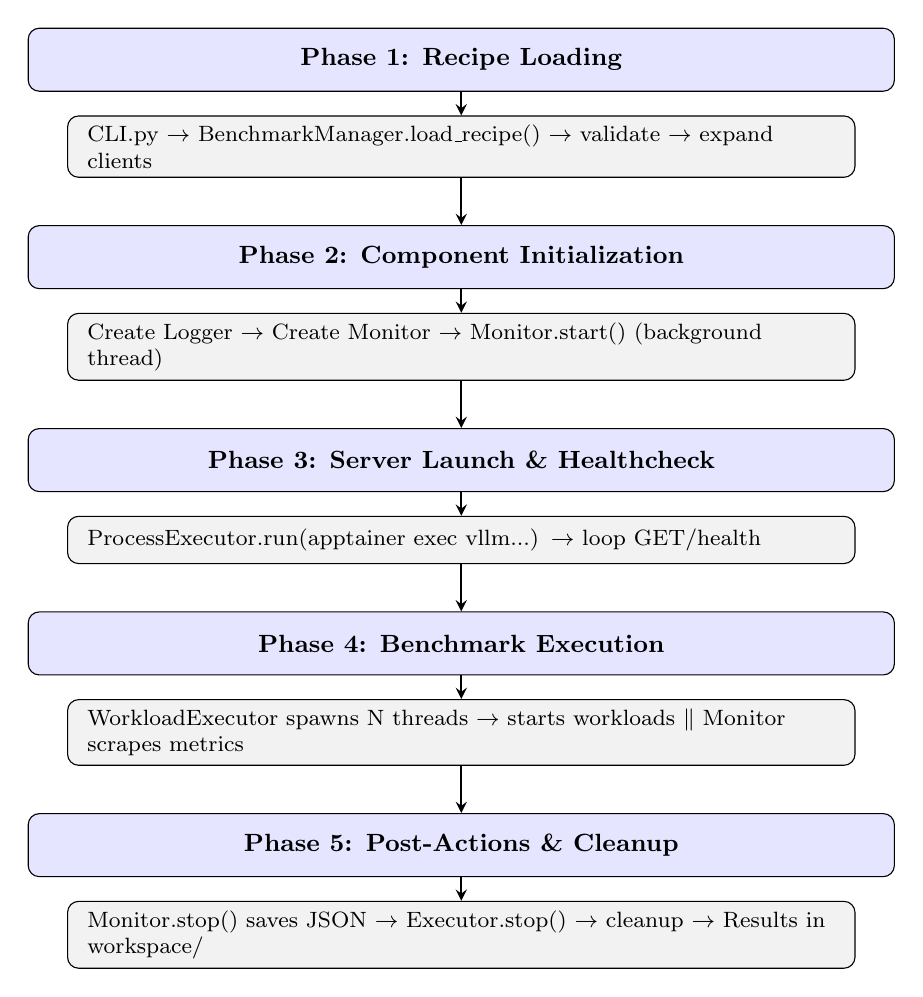
\begin{tikzpicture}[
    phase/.style={rectangle, draw, rounded corners, fill=blue!10, minimum width=11cm, minimum height=0.8cm, font=\small\bfseries},
    stepbox/.style={rectangle, draw, rounded corners, fill=gray!10, minimum width=10cm, minimum height=0.6cm, font=\footnotesize, text width=9.5cm, align=left},
    arrow/.style={->, >=stealth, thick}
]

\node[phase] (p1) {Phase 1: Recipe Loading};
\node[stepbox, below=0.3cm of p1] (s1) {CLI.py $\rightarrow$ BenchmarkManager.load\_recipe() $\rightarrow$ validate $\rightarrow$ expand clients};

\node[phase, below=0.6cm of s1] (p2) {Phase 2: Component Initialization};
\node[stepbox, below=0.3cm of p2] (s2) {Create Logger $\rightarrow$ Create Monitor $\rightarrow$ Monitor.start() (background thread)};

\node[phase, below=0.6cm of s2] (p3) {Phase 3: Server Launch \& Healthcheck};
\node[stepbox, below=0.3cm of p3] (s3) {ProcessExecutor.run(apptainer exec vllm...) $\rightarrow$ loop GET/health};

\node[phase, below=0.6cm of s3] (p4) {Phase 4: Benchmark Execution};
\node[stepbox, below=0.3cm of p4] (s4) {WorkloadExecutor spawns N threads $\rightarrow$ starts workloads $\parallel$ Monitor scrapes metrics};

\node[phase, below=0.6cm of s4] (p5) {Phase 5: Post-Actions \& Cleanup};
\node[stepbox, below=0.3cm of p5] (s5) {Monitor.stop() saves JSON $\rightarrow$ Executor.stop() $\rightarrow$ cleanup $\rightarrow$ Results in workspace/};

\draw[arrow] (p1) -- (s1);
\draw[arrow] (s1) -- (p2);
\draw[arrow] (p2) -- (s2);
\draw[arrow] (s2) -- (p3);
\draw[arrow] (p3) -- (s3);
\draw[arrow] (s3) -- (p4);
\draw[arrow] (p4) -- (s4);
\draw[arrow] (s4) -- (p5);
\draw[arrow] (p5) -- (s5);

\end{tikzpicture}
\caption{Five-phase benchmark execution flow: Recipe Loading, Component Initialization, Server Launch, Benchmark Execution, and Post-Actions.}
\label{fig:sequence}
\end{figure}

\textbf{Phase 1: Recipe Loading.} The \texttt{BenchmarkManager.load\_recipe()} method parses the YAML file, expands environment variables, validates required sections, and expands client instances.

\textbf{Phase 2: Component Initialization.} Factory methods instantiate monitors, loggers, executors, servers, and clients. Monitors begin background scraping threads.

\textbf{Phase 3: Server Launch.} Each server's \texttt{start\_service()} executes via the assigned executor. The manager polls HTTP health endpoints until servers report ready or timeout expires.

\textbf{Phase 4: Benchmark Execution.} Client instances start, spawning concurrent worker threads. The main loop polls client status at configured intervals. Prometheus monitors scrape metrics concurrently.

\textbf{Phase 5: Post-Actions.} Upon duration expiry, the manager executes \texttt{collect\_metrics} and \texttt{stop\_services}, persists metrics, and performs cleanup.

%%%%%%%%%%%%%%%%%%%%%%%%%%%%%%%%%%%%%%%%%%%%%%%%%%%%%%%%%%%%%%%%%%%%%%%%%%%%%
% SECTION 5: IMPLEMENTATION DETAILS
%%%%%%%%%%%%%%%%%%%%%%%%%%%%%%%%%%%%%%%%%%%%%%%%%%%%%%%%%%%%%%%%%%%%%%%%%%%%%
\section{Implementation Details}
\label{sec:implementation}

\subsection{Technology Stack}

\begin{table}[H]
\centering
\caption{Technology stack and dependencies}
\label{tab:tech-stack}
\begin{tabular}{@{}lll@{}}
\toprule
\textbf{Category} & \textbf{Technology} & \textbf{Version} \\
\midrule
Language & Python & 3.9+ \\
Configuration & PyYAML & $\geq$ 6.0 \\
Metrics & prometheus\_client & $\geq$ 0.17.0 \\
S3 Client & boto3 & $\geq$ 1.28.0 \\
Container Runtime & Apptainer & 1.2+ \\
Scheduler & SLURM & 21.08+ \\
\bottomrule
\end{tabular}
\end{table}

\subsection{Error Handling Strategy}

The framework implements defense-in-depth error handling:

\textbf{Healthcheck Timeout:} Polling loop with configurable retry interval. Timeout raises \texttt{TimeoutError}, triggering graceful shutdown.

\textbf{Executor Stop Isolation:} \texttt{Service.stop()} wraps executor termination in try-except, preventing cascading failures.

\textbf{Workload Error Backoff:} Worker threads increment consecutive error counters; exceeding threshold aborts the worker. Configurable backoff delay between retries.

\textbf{Monitor Resilience:} \texttt{collect()} catches all HTTP exceptions, storing error messages rather than crashing.

\subsection{Extensibility: Adding New Workloads}

To add a new workload type (e.g., ChromaDB):

\textbf{Step 1:} Create \texttt{src/Core/workloads/chromadb\_query.py} with a \texttt{run(config, logger, stop\_event)} function.

\textbf{Step 2:} Register in \texttt{WORKLOAD\_REGISTRY} dictionary in \texttt{workloads/\_\_init\_\_.py}.

\textbf{Step 3:} Create a recipe YAML with the new workload type.

%%%%%%%%%%%%%%%%%%%%%%%%%%%%%%%%%%%%%%%%%%%%%%%%%%%%%%%%%%%%%%%%%%%%%%%%%%%%%
% SECTION 6: EXPERIMENTAL SETUP
%%%%%%%%%%%%%%%%%%%%%%%%%%%%%%%%%%%%%%%%%%%%%%%%%%%%%%%%%%%%%%%%%%%%%%%%%%%%%
\section{Experimental Setup and Methodology}
\label{sec:methodology}

\subsection{MeluXina Environment}

\begin{table}[H]
\centering
\caption{MeluXina hardware specifications (GPU partition)}
\label{tab:meluxina-hw}
\begin{tabular}{@{}ll@{}}
\toprule
\textbf{Component} & \textbf{Specification} \\
\midrule
GPU Nodes & 200 nodes \\
GPUs per Node & 4$\times$ NVIDIA A100-40 \\
CPUs per Node & 2$\times$ AMD Rome (32 cores) \\
Memory per Node & 512 GB \\
Interconnect & HDR InfiniBand \\
\bottomrule
\end{tabular}
\end{table}

%%%%%%%%%%%%%%%%%%%%%%%%%%%%%%%%%%%%%%%%%%%%%%%%%%%%%%%%%%%%%%%%%%%%%%%%%%%%%
% SECTION 7: RESULTS
%%%%%%%%%%%%%%%%%%%%%%%%%%%%%%%%%%%%%%%%%%%%%%%%%%%%%%%%%%%%%%%%%%%%%%%%%%%%%
\section{Results and Performance Analysis}
\label{sec:results}

This section presents the experimental results from two benchmark scenarios executed on MeluXina: vLLM inference serving and MinIO S3 object storage. Metrics were collected via Prometheus scraping and visualized through Grafana dashboards.

\subsection{Metrics Visualization Infrastructure}

The framework includes a FastAPI-based visualization server (\texttt{src/Interface/fastapi\_server.py}) that implements the Grafana SimpleJSON datasource protocol. This enables real-time metrics visualization without external dependencies.

Key features of the visualization server:
\begin{itemize}[noitemsep]
    \item \textbf{Auto-detection:} Automatically detects service type (vLLM, MinIO) from metric prefixes
    \item \textbf{Rate calculation:} Applies \texttt{rate()} to counter metrics (\texttt{\_total}, \texttt{\_count}) automatically
    \item \textbf{Recommended metrics:} Provides service-specific default metrics for optimal dashboards
    \item \textbf{Histogram support:} Parses bucket metrics for heatmap visualizations
\end{itemize}

\subsection{vLLM Inference Benchmark Results}

The vLLM benchmark was executed on December 31, 2025, using the facebook/opt-125m model with 2 client instances (4 threads each).

\begin{table}[H]
\centering
\caption{vLLM inference benchmark configuration and results}
\label{tab:vllm-results}
\begin{tabular}{@{}ll@{}}
\toprule
\textbf{Parameter} & \textbf{Value} \\
\midrule
Model & facebook/opt-125m \\
Client Instances & 2 (4 threads each) \\
Benchmark Duration & 120 seconds \\
\midrule
Total Requests & $\approx$ 7,400 \\
Success Rate & 99.9\% \\
Average Latency & 122--130 ms \\
Throughput & $\approx$ 62 req/s \\
Concurrent Requests & 6--8 (average) \\
\bottomrule
\end{tabular}
\end{table}

Figure~\ref{fig:grafana-vllm} shows the Grafana dashboard for the vLLM benchmark. Panel 1 displays the HTTP request duration count (rate-transformed), demonstrating consistent throughput around 60--66 requests per second. Panel 2 shows the number of concurrent requests running in the vLLM engine, fluctuating between 4--8 during load. Panel 3 presents a heatmap of request latency distribution, with the majority of requests completing in the lower latency buckets (green/blue regions).

\begin{figure}[H]
\centering
\includegraphics[width=\textwidth]{diagrams/grafana_vllm.png}
\caption{Grafana dashboard for vLLM inference benchmark showing: (1) HTTP request rate, (2) concurrent requests running, (3) latency distribution heatmap.}
\label{fig:grafana-vllm}
\end{figure}

\subsection{MinIO S3 Storage Benchmark Results}

The S3 benchmark was executed using MinIO as the object storage backend, testing upload and download operations with varying object sizes.

\begin{table}[H]
\centering
\caption{MinIO S3 benchmark configuration and results}
\label{tab:s3-results}
\begin{tabular}{@{}ll@{}}
\toprule
\textbf{Parameter} & \textbf{Value} \\
\midrule
Storage Backend & MinIO (containerized) \\
Client Instances & 4 \\
Benchmark Duration & 300 seconds \\
\midrule
Peak Request Rate & $\approx$ 60--70 req/s \\
Traffic Sent & 400--700 MB/interval \\
TTFB Distribution & Consistent across buckets \\
\bottomrule
\end{tabular}
\end{table}

Figure~\ref{fig:grafana-s3} presents the MinIO benchmark dashboard. Panel 1 shows the total S3 requests over time with multiple client streams (color-coded). Panel 2 displays traffic sent in bytes, showing periodic bursts corresponding to batch uploads. Panel 3 provides a heatmap of Time-To-First-Byte (TTFB) latency distribution across histogram buckets.

\begin{figure}[H]
\centering
\includegraphics[width=\textwidth]{diagrams/grafana_s3.png}
\caption{Grafana dashboard for MinIO S3 benchmark showing: (1) total requests per client, (2) traffic sent bytes, (3) TTFB seconds distribution heatmap.}
\label{fig:grafana-s3}
\end{figure}

\subsection{Output Data Structure}

Benchmark results are persisted in timestamped directories with the following structure:
\begin{itemize}[noitemsep]
    \item \texttt{logs/} -- JSON-lines application logs
    \item \texttt{slurm\_logs/} -- SLURM stdout/stderr from job execution
    \item \texttt{*\_metrics.json} -- Raw Prometheus scrapes (text format)
    \item \texttt{*\_metrics\_parsed.json} -- Structured JSON with metric names, labels, and values
\end{itemize}

%%%%%%%%%%%%%%%%%%%%%%%%%%%%%%%%%%%%%%%%%%%%%%%%%%%%%%%%%%%%%%%%%%%%%%%%%%%%%
% SECTION 8: CONCLUSION
%%%%%%%%%%%%%%%%%%%%%%%%%%%%%%%%%%%%%%%%%%%%%%%%%%%%%%%%%%%%%%%%%%%%%%%%%%%%%
\section{Conclusion and Future Work}
\label{sec:conclusion}

\subsection{Achievements}

This project delivered a production-ready benchmarking framework:

\begin{enumerate}[noitemsep]
    \item Modular four-module architecture with abstract base classes for extensibility.
    \item First-class SLURM support with Apptainer containerization.
    \item YAML-based Recipe specifications for reproducibility.
    \item Prometheus-compatible monitoring with parsed JSON output.
    \item Validated object storage and vLLM inference.
\end{enumerate}

\subsection{Future Work}

\begin{itemize}[noitemsep]
    \item Extended workload suite (vector DBs).
    \item Multi-node scaling with distributed client load generation.
    \item Workflow DAG support for multi-stage benchmarks.
    \item Real-time web dashboard for live monitoring.
\end{itemize}

%%%%%%%%%%%%%%%%%%%%%%%%%%%%%%%%%%%%%%%%%%%%%%%%%%%%%%%%%%%%%%%%%%%%%%%%%%%%%
% REFERENCES
%%%%%%%%%%%%%%%%%%%%%%%%%%%%%%%%%%%%%%%%%%%%%%%%%%%%%%%%%%%%%%%%%%%%%%%%%%%%%
\section*{References}

\begin{enumerate}[label={[\arabic*]}]
    \item EuroHPC Joint Undertaking. \url{https://eurohpc-ju.europa.eu/}
    \item LuxProvide MeluXina. \url{https://luxprovide.lu/meluxina/}
\end{enumerate}

\end{document}
